\documentclass[11pt]{article}
\usepackage[margin=1in]{geometry}
\usepackage{amsmath,amssymb,amsthm}
\usepackage{enumitem}
\usepackage[T1]{fontenc}
\usepackage{lmodern}
\usepackage{graphicx}
\usepackage{booktabs}
\usepackage{hyperref}
\hypersetup{colorlinks=true,linkcolor=black,citecolor=black,urlcolor=blue}
\makeatletter\g@addto@macro\UrlBreaks{\do\_}\makeatother

\newtheorem{theorem}{Theorem}[section]
\newtheorem{lemma}[theorem]{Lemma}
\newtheorem{proposition}[theorem]{Proposition}
\newtheorem{corollary}[theorem]{Corollary}
\newtheorem{law}[theorem]{Law}
\theoremstyle{definition}
\newtheorem{definition}[theorem]{Definition}
\newtheorem{computation}[theorem]{Computation}
\theoremstyle{remark}
\newtheorem{remark}[theorem]{Remark}

\newcommand{\N}{\mathbb{N}}
\newcommand{\F}{\mathbb{F}_2}
\newcommand{\PROVED}{\textsc{Proved}}
\newcommand{\EXACT}{\textsc{Exact}}
\newcommand{\MEASURED}{\textsc{Measured}}
\newcommand{\KNOWN}{\textsc{Known}}
\newcommand{\OPEN}{\textsc{Open}}
\newcommand{\dstar}{d^{*}}

\title{The left edge of Rule~30 without Rule~30:\\ the stripe recursion, Wolfram's number $2{,}107{,}985{,}255$,\\ and the forks beyond it}
\author{N.~Berzai\thanks{Computational and editorial assistance from Claude (Anthropic). Every numbered result carries a status label, defined in Section~1; no claim is made beyond its label.}}
\date{30 September 2026; revised 7 October 2026}

\begin{document}
\maketitle

\begin{abstract}
The left edge of the Rule~30 pattern grown from one black cell is made of diagonals that become periodic, with periods that are powers of two. Wolfram tabulated the depths at which the period first reaches $2,4,8,16,32$ and gave the sixth, where it reaches $64$, as ``$2{,}107{,}985{,}255$ or more''. The eventual patterns of consecutive diagonals obey a two-term recursion with a closed form, which we run without simulating the rule; it is deterministic except at a diagonal that ends all white, where it forks. The eighth such diagonal of the seed is $d=1{,}420{,}878{,}968$, a genuine fork: on one branch the period reaches $64$ at exactly $d=2{,}107{,}985{,}255$, on the other not below $3.34\cdot10^9$. This fork and this onset were, to our knowledge, first made public on 8 September 2026 in two independent code repositories \cite{Dib,Pat}; we obtained the same integers independently on 24 September 2026. Beyond the doubling the first branch has no further fork up to $10^{12}$. Over more than $10^{10}$ pairs, consecutive patterns differ in a binomially distributed number of cells; if this holds down to distance $0$, forks come about once per $2^P$ diagonals at period $P$ and the next doubling lies near $10^{19}$--$10^{20}$, beyond any computation. We prove that at a fork the order--chaos front advances exactly when the frozen diagonal is black on the row after the previous front, and that, given the front's path over the three preceding diagonals, five cells of the last three patterns force the seed onto the branch of Wolfram's number. That path is the one input not proved; it is the same in all eight coin-driven models of the front whose path we recorded across the fork, and all twenty-eight models we ran take that branch. The centre column the stripes alone would produce passes every fair-coin test we applied to $10^9$ bits but one, and the real centre column is that sequence XOR a transient bit that behaves, in every test we ran, as an independent coin.
\end{abstract}

\section{Introduction}

Rule~30 started from a single black cell produces a pattern whose right side looks random and whose left side is striped: each diagonal parallel to the left edge becomes periodic after a transient, with a period that is a power of two \cite{GG,Jen86,Rowland}. The period of the stripes grows. Wolfram \cite[p.~871]{NKS} lists the depths at which the maximal period first reaches $2,4,8,16,32$ as $3,8,29,400,87{,}867$ and the sixth, period $64$, as ``$2{,}107{,}985{,}255$ or more''. Gravner and Griffeath \cite[\S8]{GG} describe the eventual patterns as the labels of a tree and record that ``the first genuine branching occurs for period 16 at generation 53{,}207''.

This note does four things.
\begin{enumerate}[leftmargin=*,itemsep=1pt]
\item It writes the recursion between consecutive eventual patterns in closed form (Lemma~\ref{lem:rec}) and runs it forward in C at about $3\cdot10^7$ diagonals a second on one core, with no simulation of the rule. The recursion forks only at a diagonal that ends all white.
\item It recomputes the eighth such diagonal of the seed, $\dstar=1{,}420{,}878{,}968$, a genuine fork, on which one branch doubles the period at Wolfram's number to the digit while the other does not double below $3.34\cdot10^9$ (Theorem~\ref{thm:eighth}). These integers were public before this note \cite{Dib,Pat}; the attribution is at the end of this section. It adds that the branch of Wolfram's number has no further fork up to $10^{12}$ (Theorem~\ref{thm:frontier}).
\item It gives the measured reason why a seventh doubling is out of reach: consecutive patterns differ binomially, so forks come about once per $2^P$ diagonals at period $P$, which matches the spacing of the doublings (Law~\ref{law:fork}).
\item It shows what decides which branch the picture takes. At a diagonal that ends all white the front between the striped and the chaotic region advances exactly when that diagonal is black on the row after the previous front (Theorem~\ref{thm:advance}), and in the cases met at the seed's forks this fixes the branch. For the seed at $\dstar$ a five-line derivation gives the branch of Wolfram's number from five pattern cells and the front's path modulo $32$ over the three preceding diagonals (Theorem~\ref{thm:seedbranch}).
\end{enumerate}
The one input not proved is that path, which every coin-driven model of the front that we recorded shares; we isolate it as the first open problem. The recursion itself is the forward form of the label tree of Gravner and Griffeath \cite{GG}, and its closed form is the reset formula of \cite{B}, the closed form of any eventually periodic diagonal, applied to the eventual patterns; the parity rule at a frozen diagonal is Rowland's \cite{Rowland}, and that the two branches at a doubling are translates is in \cite[\S8]{GG}. Running the recursion forward in place of the rule is not new either: two code repositories did so before us, past $\dstar$. The eighth frozen diagonal, $\dstar=1{,}420{,}878{,}968$, and the period-$64$ onset at $2{,}107{,}985{,}255$ on one of its two branches were, to our knowledge, first made public on 8 September 2026 in two independent code repositories: Dibujaron/rule30 \cite{Dib} and Patto1155/rule30-foundry \cite{Pat}, the second from a run of about 30 August 2026. We obtained the same integers independently on 24 September 2026 and learned of these repositories on 1 October 2026. We found the numbers in no paper, preprint or OEIS entry. The second repository also follows both branches at every fork up to $1.2\cdot10^{10}$; the only other period-$64$ onset it records is at $9{,}958{,}700{,}505$, on the other side of the fork. Neither repository determines which branch the seed takes, and neither do we. What we have not found elsewhere, to our knowledge, is the reading of Wolfram's number as the smallest onset over the branches (Remark~\ref{rem:ormore}), the absence of a further fork on the branch of Wolfram's number up to $10^{12}$ (Theorem~\ref{thm:frontier}), the binomial fork law (Law~\ref{law:fork}), the advance criterion and the conditional derivation of the seed's branch (Theorems~\ref{thm:advance} and~\ref{thm:seedbranch}), and the edge-machine evidence (Computation~\ref{comp:vote}). The note is self-contained: the facts about the front that its proofs use are proved in Section~\ref{sec:setting}. Our longer manuscript \cite{B} is cited only for context. Results carry a status: \PROVED; \EXACT\ for a finite computation reproducible from the accompanying code; \MEASURED\ for a statistical statement; \KNOWN\ for the literature; \OPEN.

\section{Setting}\label{sec:setting}

Rule~30 is $u^{t+1}_x=u^t_{x-1}\oplus(u^t_x\vee u^t_{x+1})$ on $x\in\mathbb Z$, from $u^0_x=[x=0]$. The \emph{diagonal frame} is $D_d(t)=u^t_{d-t}$ for $d,t\ge0$: diagonal $d=0$ is the left edge $x=-t$, which is always black. In this frame the rule reads
\begin{equation}\label{eq:frame}
D_{d+1}(t+1)=D_{d-1}(t)\oplus\bigl(D_d(t)\vee D_{d+1}(t)\bigr)\qquad(d,t\ge0,\ D_{-1}\equiv0).
\end{equation}
Every $D_d$ is eventually periodic with minimal period $p_d$ a power of two \cite{Jen86,GG,Rowland}. Let $r_d\colon\N\to\F$ be the periodic sequence with $D_d(t)=r_d(t)$ for all large $t$ (the \emph{label} of diagonal $d$), $\tau_d$ the least $\tau$ with $D_d(t)=r_d(t)$ for all $t\ge\tau$, and $\Delta_d=D_d\oplus r_d$ the \emph{defect}, which has finite support ending at row $\tau_d-1$ (empty if $\tau_d=0$). The \emph{front} is $M_d=\max(\tau_{d-1},\tau_d)-1$, the last row on which diagonal $d-1$ or $d$ is still transient. We say row $t$ lies \emph{beyond the front} of diagonal $d$ if $t\ge M_d+1$; there both $D_{d-1}(t)=r_{d-1}(t)$ and $D_d(t)=r_d(t)$. Diagonal $d$ is \emph{frozen} if $r_d\equiv0$, that is, if it ends all white. The front \emph{moves} (or advances) at $d$ if $M_d>M_{d-1}$, and \emph{stalls} at $d$ otherwise. We call the sequence of labels the \emph{wall}, and a sequence of labels generated by the recursion of Section~3, with a choice made at each fork, a \emph{lineage}. Figure~\ref{fig:edge} shows the picture.

The diagonal $d=0$ is black on every row: $u^{t}_{-t}=u^{t-1}_{-t-1}\oplus(u^{t-1}_{-t}\vee u^{t-1}_{-t+1})=0\oplus(0\vee1)=1$ by induction, so $r_0\equiv1$ and $\tau_0=0$. The rest of what the proofs below use about labels and fronts is the following.

\begin{lemma}[labels and the front; \PROVED]\label{lem:front}
\begin{enumerate}[label=(\alph*),leftmargin=*,itemsep=1pt]
\item \emph{Background equation.} $r_{d+1}(t+1)=r_{d-1}(t)\oplus\bigl(r_d(t)\vee r_{d+1}(t)\bigr)$ for all $d\ge0$ and all $t$, with $r_{-1}\equiv0$ and the labels extended periodically to all integers.
\item No two consecutive labels are both zero.
\item \emph{Monotonicity.} $M_d\le M_{d+1}$.
\item \emph{Landing rule.} Either $M_{d+1}=M_d$, or diagonal $d$ is not frozen and $M_{d+1}=n:=\min\{t\ge M_d+1: r_d(t)=1\}$, the first black cell of $r_d$ beyond the front; in the second case the defect of diagonal $d+1$ is $1$ on the rows $M_d+1,\dots,n$ and ends there, $\tau_{d+1}-1=M_{d+1}=n$.
\item If diagonal $d$ is frozen, $M_{d+1}=M_d$.
\end{enumerate}
\end{lemma}

\begin{proof}
(a) For $t$ beyond $\tau_{d-1},\tau_d,\tau_{d+1}$ the three diagonals equal their labels and \eqref{eq:frame} reads as stated; both sides are periodic in $t$, so the identity holds for all $t$.
(b) Suppose $r_{d-1}=r_d\equiv0$ with $d\ge1$. Then (a) with $d-1$ in place of $d$ gives $0=r_d(t+1)=r_{d-2}(t)$, so $r_{d-2}\equiv0$ too, and descending, $r_0\equiv0$, which is false. (This is the argument of \cite[Proposition~3.3]{GG}.)
(c), (d), (e) Subtracting (a) from \eqref{eq:frame} gives, for every $t$,
\[
\Delta_{d+1}(t+1)=\Delta_{d-1}(t)\oplus\bigl(D_d(t)\vee D_{d+1}(t)\bigr)\oplus\bigl(r_d(t)\vee r_{d+1}(t)\bigr).
\]
If $t\ge\tau_d$ and $t\ge\tau_{d+1}$ the last two terms cancel, so $\Delta_{d-1}(t)=\Delta_{d+1}(t+1)=0$ for $t\ge\max(\tau_d,\tau_{d+1})$: hence $\tau_{d-1}\le\max(\tau_d,\tau_{d+1})$, which is (c). For $t\ge M_d+1$ the first term vanishes and $D_d=r_d$, so, using $(x\vee a)\oplus(x\vee b)=\neg x\wedge(a\oplus b)$,
\[
\Delta_{d+1}(t+1)=\neg r_d(t)\wedge\Delta_{d+1}(t)\qquad(t\ge M_d+1).
\]
If $r_d\equiv0$ the defect $\Delta_{d+1}$ is constant from row $M_d+1$ on, hence $0$ there, so $\tau_{d+1}\le M_d+1$ and, with (c), $M_{d+1}=M_d$: this is (e). Otherwise $\Delta_{d+1}$ keeps its value $\Delta_{d+1}(M_d+1)$ on the rows $M_d+1,\dots,n$, where $r_d$ is white, and is $0$ from row $n+1$ on. If that value is $0$ then $\tau_{d+1}\le M_d+1$ and $M_{d+1}=M_d$ by (c). If it is $1$ then $\tau_{d+1}=n+1$, so $M_{d+1}=\max(\tau_d,n+1)-1=n$, since $n\ge M_d+1\ge\tau_d$. This is (d).
\end{proof}

In every case examined, the labels of a left half of Rule~30, driven by its boundary column from a finite initial state, are the seed's up to a translation of rows: this is \KNOWN\ for every finite seed up to diagonal $53{,}207$ \cite[\S8]{GG}, and \EXACT\ for seven combinations of boundary column, some random, and initial state up to diagonal $12{,}000$ \cite{B}. We use this only as a measured hypothesis, in Proposition~\ref{prop:phase}.

\begin{figure}[t]
\centering
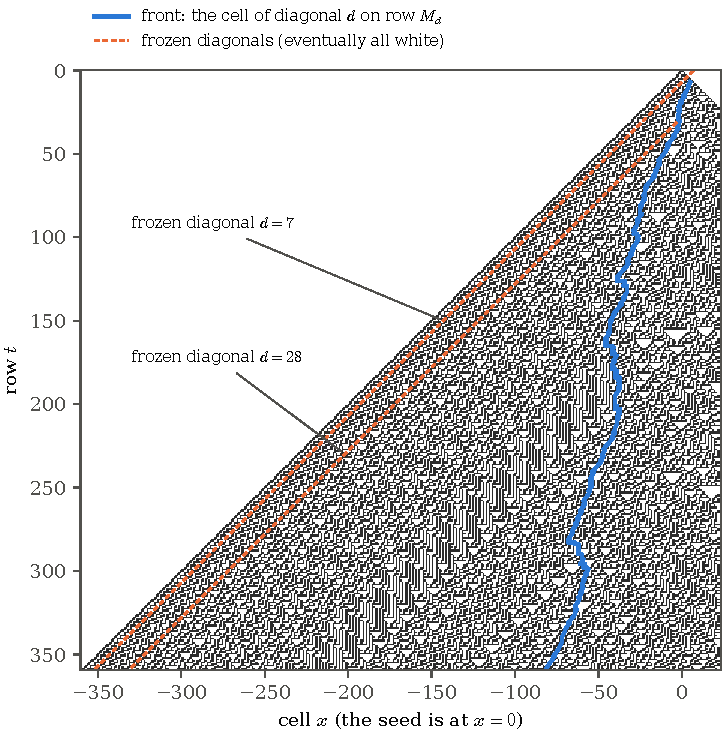
\includegraphics[width=0.6\textwidth]{figures/fig_left_edge.pdf}
\caption{The left edge of Rule~30 from one cell, rows $0$--$359$. Diagonals run from upper right to lower left. Left of the blue front each diagonal is periodic (the stripes); right of it the pattern is still transient. The frozen diagonals $d=7$ and $d=28$ are all white from rows $0$ and $31$ on (dashed); $d=2$, white from row $2$ on, runs along the edge and is not marked. Here the front leans left by about $0.2$ cells per row; over the first $800{,}000$ diagonals its average lean is $0.24$.}
\label{fig:edge}
\end{figure}

\section{The stripe recursion}

\begin{lemma}[\PROVED]\label{lem:rec}
Let $(a,b)=(r_{d-1},r_d)$ and $c=r_{d+1}$. Then $c(t+1)=a(t)\oplus b(t)\oplus\bigl(\neg b(t)\wedge c(t)\bigr)$ for all $t$.
\begin{enumerate}[label=(\alph*),leftmargin=*,itemsep=1pt]
\item If $b\not\equiv0$, extend $a,b,c$ periodically to all integers and let $u^*<t$ be the last row before $t$ with $b(u^*)=1$. Then $c(t)=a(u^*)\oplus1\oplus\bigoplus_{u^*<s<t}a(s)$. So $c$ is the unique periodic solution, and its period divides $\operatorname{lcm}(p_{d-1},p_d)$.
\item If $b\equiv0$ (diagonal $d$ is frozen), $c(t)=c(0)\oplus\bigoplus_{0\le s<t}a(s)$ for $t\ge0$. Both solutions are periodic, and they are complements. Their minimal period is $p_{d-1}$ if $a$ has even weight on a period and $2p_{d-1}$ if odd.
\end{enumerate}
\end{lemma}

\begin{proof}
The recursion is Lemma~\ref{lem:front}(a), since $b\vee c=b\oplus(\neg b\wedge c)$. Where $b(s)=1$ the recursion gives $c(s+1)=a(s)\oplus1$ whatever $c(s)$ was; where $b(s)=0$ it gives $c(s+1)=a(s)\oplus c(s)$. Iterating from $u^*$ gives (a). Every solution agrees with (a) after the first black cell of $b$, so the periodic one is unique and inherits every common period of $a$ and $b$. In (b), $c(t+p)=c(t)\oplus\bigoplus_{s=t}^{t+p-1}a(s)$ for $p=p_{d-1}$, which is $c(t)$ at even weight and $\neg c(t)$ at odd weight. Since $a(t)=c(t)\oplus c(t+1)$, every period of $c$ is a period of $a$, so the minimal period of $c$ is $p$ at even weight and $2p$ at odd weight.
\end{proof}

Lemma~\ref{lem:rec} is that reset formula applied to the labels, and part (b) is Rowland's parity law \cite{Rowland}. The recursion also runs backwards: $a(t)=c(t+1)\oplus b(t)\oplus(\neg b(t)\wedge c(t))$ recovers $r_{d-1}$ from $(r_d,r_{d+1})$, so each pair of consecutive labels has exactly one predecessor pair, and this \emph{backward map} commutes with translation of rows. Read backwards, the wall is the tree of Gravner and Griffeath \cite{GG}.

\begin{corollary}[\PROVED]\label{cor:forks}
(i) Diagonal $d\ge2$ is frozen if and only if $r_{d-2}=r_{d-1}$: forks are twins.
(ii) The running maximum of $p_d$ grows only across a frozen diagonal, from $d-1$ to $d+1$, and then by a factor of two.
(iii) At a frozen diagonal whose predecessor label has odd weight, the two candidates are translates of each other by $p_{d-1}$ rows. At each frozen diagonal of Table~\ref{tab:frozen} where it has even weight, no translation maps one candidate to the other, so the branches are different walls.
\end{corollary}

\begin{proof}
(i) Put $c\equiv0$ in the recursion: $a=b$. Conversely if $a=b\not\equiv0$ then (a) gives $c(t)=a(u^*)\oplus1\oplus0=0$; and $a=b\equiv0$ cannot occur by Lemma~\ref{lem:front}(b). (ii) By Lemma~\ref{lem:rec}(a), $p_{d+1}\le\max(p_{d-1},p_d)$ unless $d$ is frozen; if it is, $p_{d+1}\le2p_{d-1}$ by (b), and $2p_{d-1}$ exceeds the running maximum only if $p_{d-1}$ equals it. (iii) At odd weight $c(t+p_{d-1})=\neg c(t)$, and $\neg c$ is the other candidate. At the even-weight frozen diagonals of Table~\ref{tab:frozen} the candidate weights are $4/12$ at $53{,}207$, $6/10$ at $58{,}286$ and $14/18$ at $\dstar$, so they are not translates; at $3{,}340{,}408{,}059$ both weigh $16$, and a direct check of the $32$ rotations finds none that maps one to the other. No later pair of consecutive labels on one branch is a translate of the pair of the same index on the other either: the backward map, which recovers $(r_{j-1},r_j)$ from $(r_j,r_{j+1})$, commutes with translation, so such a pair would make the candidates translates.
\end{proof}

The first statement of (iii) is in \cite[\S8]{GG}. Every frozen diagonal is a fork of the recursion; we call it a \emph{doubling} when $r_{d-1}$ has odd weight, since the period then doubles and the two branches are one wall up to translation, and a \emph{genuine fork} when the weight is even.

\emph{Validation} (\EXACT). Started from $(r_{19},r_{20})$ and given the seed's branch at each fork, the recursion reproduces the labels of a direct simulation at all $799{,}980$ diagonals up to $800{,}000$. Implementations with $64$- and $128$-bit pattern words, run from $d=90{,}000$, stop at the same frozen diagonal $\dstar$ with the same labels and the same count of diagonals of each period.

\section{The eighth frozen diagonal and Wolfram's number}

\begin{theorem}[\EXACT; made public earlier in \cite{Dib,Pat}]\label{thm:eighth}
The frozen diagonals of the seed's lineage up to the fork, and on each branch after it up to the next frozen diagonal, are those of Table~\ref{tab:frozen}. The eighth, $\dstar=1{,}420{,}878{,}968$, is a genuine fork: $r_{\dstar-1}$ has period $32$ and weight $20$, and the candidates for $r_{\dstar+1}$ are \texttt{93425cac} and \texttt{6cbda353} (bit $t$ of the $32$-bit word is the cell on row $t$ modulo $32$). On the branch \texttt{6cbda353} the next frozen diagonal is $2{,}107{,}985{,}254$, of odd weight $17$, and the period first reaches $64$ at $d=2{,}107{,}985{,}255$. On the branch \texttt{93425cac} the next frozen diagonal is $3{,}340{,}408{,}059$, of even weight $16$, and the period stays at most $32$ up to it.
\end{theorem}

\emph{Attribution.} The integers of Theorem~\ref{thm:eighth} were public before this note. The eighth frozen diagonal, $\dstar=1{,}420{,}878{,}968$, and the period-$64$ onset at $2{,}107{,}985{,}255$ on one of its two branches were, to our knowledge, first made public on 8 September 2026 in two independent code repositories. Dibujaron/rule30 \cite{Dib} gives $\dstar$ as the eighth all-white diagonal, with two complementary continuations. On one the next all-white diagonal is $2{,}107{,}985{,}254$ and the period doubles at $2{,}107{,}985{,}255$, which it identifies with Wolfram's figure. On the other the next are $3{,}340{,}408{,}059$ and $4{,}989{,}445{,}007$, with no doubling below $5.16\cdot10^9$. Patto1155/rule30-foundry \cite{Pat}, from a run of about 30 August 2026, gives the first branch point at $\dstar+1$ with the two words \texttt{93425cac} and \texttt{6cbda353}, and the doubling at $2{,}107{,}985{,}255$ on the second. It follows both branches at every fork up to $1.2\cdot10^{10}$ and records one further doubling there, at $9{,}958{,}700{,}505$, on the side of the first word. We obtained the same integers independently on 24 September 2026 and learned of these repositories on 1 October 2026. We found the numbers in no paper, preprint or OEIS entry. Neither repository determines which branch the seed takes (Section~6).

\begin{table}[t]
\centering
\small
\begin{tabular}{rrrll}
\toprule
frozen diagonal $d$ & period of $r_{d-1}$ & weight & type & new period, first at\\
\midrule
$2$ & $1$ & $1$ & doubling & $2$ at $d=3$\\
$7$ & $2$ & $1$ & doubling & $4$ at $d=8$\\
$28$ & $4$ & $3$ & doubling & $8$ at $d=29$\\
$399$ & $8$ & $3$ & doubling & $16$ at $d=400$\\
$53{,}207$ & $16$ & $6$ & genuine fork & \\
$58{,}286$ & $16$ & $10$ & genuine fork & \\
$87{,}866$ & $16$ & $5$ & doubling & $32$ at $d=87{,}867$\\
$1{,}420{,}878{,}968$ & $32$ & $20$ & genuine fork & \\
$2{,}107{,}985{,}254$\rlap{$^a$} & $32$ & $17$ & doubling & $64$ at $d=2{,}107{,}985{,}255$\\
$3{,}340{,}408{,}059$\rlap{$^b$} & $32$ & $16$ & genuine fork & \\
\bottomrule
\end{tabular}
\caption{Frozen diagonals of the seed's lineage (\EXACT), with the period and weight of $r_{d-1}$. Odd weight gives a doubling, even weight a genuine fork. The branches at $\dstar=1{,}420{,}878{,}968$ are \texttt{93425cac} and \texttt{6cbda353}; ${}^a$on the branch \texttt{6cbda353}, ${}^b$on the branch \texttt{93425cac}. The last three rows were made public earlier in \cite{Dib,Pat}; see the attribution after Theorem~\ref{thm:eighth}.}
\label{tab:frozen}
\end{table}

\begin{remark}\label{rem:ormore}
By Theorem~\ref{thm:eighth} neither branch at $\dstar$ reaches period $64$ before $2{,}107{,}985{,}255$, so that number is the smallest period-$64$ onset over the branches. Wolfram's ``$2{,}107{,}985{,}255$ or more'' is consistent with a computation of this kind that met the fork at $\dstar$ and reported the earlier of its two outcomes as a lower bound. We have not found this reading stated. The match of the onset with Wolfram's number is noted in \cite{Dib}, which infers from it that the seed takes this branch and lists that step as not checked. \cite{NKS} gives no reason for ``or more''. We do not claim to know how the number was obtained.
\end{remark}

\begin{theorem}[\EXACT]\label{thm:frontier}
Beyond $2{,}107{,}985{,}255$ the lineage of the branch \texttt{6cbda353} has no frozen diagonal up to $d=10^{12}$, so its period-$64$ regime lasts at least until $d=10^{12}$. The computation beyond $1.508\cdot10^{11}$ ran on a second machine, from a checkpoint of the first, in $8{,}492$ steps of $10^8$ diagonals. Thirteen of them, at six places up to $6.503\cdot10^{11}$, were recomputed on the first machine by two separately written programs, with $64$- and $128$-bit pattern words, and agree to the last hex digit.
\end{theorem}

The statement does not depend on the branch taken at $2{,}107{,}985{,}254$. That frozen diagonal has odd weight, so its two candidates are translates (Corollary~\ref{cor:forks}(iii)). By the uniqueness in Lemma~\ref{lem:rec}(a) the two lineages after it are then translates of each other, and being frozen is invariant under translation. Inside the regime a label occasionally has minimal period $32$, as Lemma~\ref{lem:rec}(a) allows: $188$ of the $8.492\cdot10^{11}$ labels computed on the second machine, against $197.7\pm14.1$ expected for uniformly random $64$-bit patterns.

\section{The fork law}

\begin{law}[\MEASURED]\label{law:fork}
In a regime of period $P$, the number of rows in a period where consecutive labels $r_d$ and $r_{d+1}$ differ is distributed as $\mathrm{Binomial}(P,\tfrac12)$.
\end{law}

Figure~\ref{fig:forklaw} shows the evidence. Over the $1.42\cdot10^9$ consecutive pairs of the seed's period-$32$ regime from $d=90{,}000$ to the fork, the counts fit the binomial with $\chi^2=29.7$ on the $31$ classes with expectation at least $5$ (distances $1$--$31$); at distances $0$ and $32$, where $0.33$ pairs are expected, $1$ and $0$ are seen. Over the first $10^{10}$ pairs of the period-$64$ regime they fit it with $\chi^2=51.7$ on the $47$ classes with expectation at least $5$, and on both tails: at distance $8$, $2.4$ pairs are expected and $3$ seen; at $56$ and $57$, $2.4$ and $0.3$ are expected and $1$ and $1$ seen.

By Corollary~\ref{cor:forks}(i) a frozen diagonal is the distance-$0$ class, so if the law holds down to distance $0$, frozen diagonals come at rate $2^{-P}$; the single pair at distance $0$ against $0.33$ expected at $P=32$ is all the direct evidence at that distance. Heuristically, if about half of them have odd weight, as for independent uniform patterns, about half end the regime, and the expected length of a period-$P$ regime is about $2^{P+1}$ diagonals: $1.3\cdot10^5$ at $P=16$, $8.6\cdot10^9$ at $P=32$, $3.7\cdot10^{19}$ at $P=64$. The seed's period-$16$ regime is $87{,}467$ long with three frozen diagonals; on the branch of Wolfram's number its period-$32$ regime is $2.1\cdot10^9$ long with two. Both are within Poisson scatter of these values. So a period of $128$ is expected near $10^{19}$--$10^{20}$ diagonals, and if the seed takes that branch (Theorem~\ref{thm:seedbranch}), $2{,}107{,}985{,}255$ is the last doubling of its left edge within reach of computation.

\begin{figure}[t]
\centering
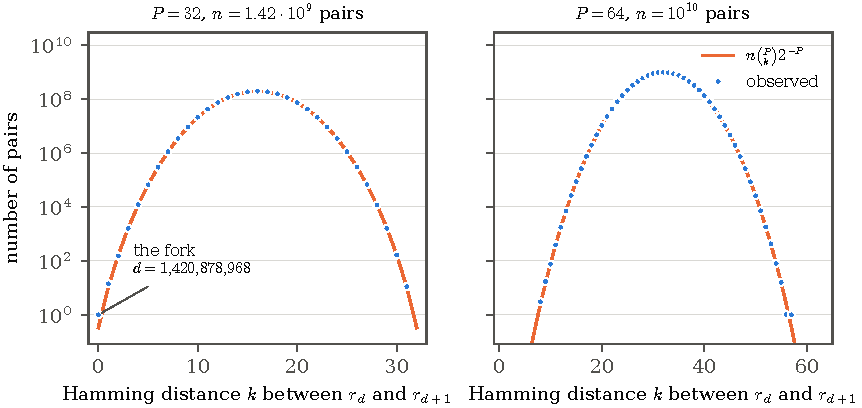
\includegraphics[width=0.94\textwidth]{figures/fig_fork_law.pdf}
\caption{The fork law. Number of consecutive label pairs at Hamming distance $k$ (dots) against $n\binom Pk2^{-P}$ (line). Left: the period-$32$ regime of the seed from $d=90{,}000$ to the fork; the single pair at $k=0$ is the fork $\dstar$. Right: the first $10^{10}$ pairs of the period-$64$ regime.}
\label{fig:forklaw}
\end{figure}

The law is the wall's own pseudo-randomness statement: the orbit of the recursion on the $4^P$ label pairs looks, in the distances between consecutive labels, like a sequence of independent uniform patterns. What is proved is only its link to the forks, Corollary~\ref{cor:forks}(i). We know no route to a proof of the law itself, which would need a mixing property of the recursion's orbit.

\section{Which branch the picture takes}

Which branch the seed takes at $\dstar$ is, to our knowledge, not determined in any public source. The two repositories that made the fork public both leave it open: \cite{Pat} records the branch of the actual diagonal as unresolved, and \cite{Dib} infers the seed's branch from the match with Wolfram's number and lists that step as not checked. This section does not determine it either. It proves what decides the branch at a frozen diagonal, and it derives the seed's branch at $\dstar$ from one hypothesis that is measured, not proved (Theorem~\ref{thm:seedbranch}).

\begin{theorem}[branch rule; \PROVED]\label{thm:branch}
Let $d$ be frozen with $\tau_d\ge1$, so $D_d(t)=0$ for $t\ge\tau_d$ and $D_d(\tau_d-1)=1$. Then $D_{d+1}(\tau_d)=D_{d-1}(\tau_d-1)\oplus1$ and $D_{d+1}(t+1)=D_{d-1}(t)\oplus D_{d+1}(t)$ for $t\ge\tau_d$. The label taken is the candidate with
\[
r_{d+1}(\tau_d-1)=1\oplus\bigoplus_{t\ge\tau_d-1}\Delta_{d-1}(t).
\]
The branch is fixed by the cells of diagonal $d-1$ from row $\tau_d-1$ on.
\end{theorem}

\begin{proof}
Apply \eqref{eq:frame} at row $\tau_d-1$, where $D_d=1$ forces the OR to $1$, and at rows $t\ge\tau_d$, where $D_d=0$ leaves $D_{d+1}(t)$. Both candidates $c$ satisfy $c(t+1)=r_{d-1}(t)\oplus c(t)$. Subtracting, $\Delta_{d+1}(t+1)=\Delta_{d-1}(t)\oplus\Delta_{d+1}(t)$ for $t\ge\tau_d$, so $\Delta_{d+1}$ is eventually the constant $\Delta_{d+1}(\tau_d)\oplus\bigoplus_{t\ge\tau_d}\Delta_{d-1}(t)$, which must vanish. Expanding $\Delta_{d+1}(\tau_d)$ with the first identity and the candidate recursion at row $\tau_d-1$ gives the displayed condition.
\end{proof}

\begin{theorem}[advance criterion; \PROVED]\label{thm:advance}
Let $d\ge2$ be frozen and $m=M_{d-1}$. From row $m+1$ on, $D_d$ keeps its value until the first black cell of $r_{d-1}$ at or after $m+1$, and is white after it. Hence the front advances at $d$ if and only if $D_d(m+1)=1$. It then lands on $\min\{t\ge m+1:r_{d-1}(t)=1\}$ and the branch taken has $r_{d+1}(M_d+1)=0$. Otherwise $M_d=m$.
If the front moved at $d-1$, the criterion reads: the front stalls at $d$ if and only if $D_d(m)=1$, and then the branch taken has $r_{d+1}(m)=0$. In that case a black cell of $r_{d-3}$ strictly between the last two landing rows $M_{d-2}$ and $m$ forces the stall.
\end{theorem}

\begin{proof}
By Corollary~\ref{cor:forks}(i), $r_{d-2}=r_{d-1}=:r$. For $t\ge m+1$ both $D_{d-2}(t)$ and $D_{d-1}(t)$ equal $r(t)$, since $t$ lies beyond the front $M_{d-1}=m$. So \eqref{eq:frame} gives $D_d(t+1)=r(t)\oplus(r(t)\vee D_d(t))$, which is $0$ where $r(t)=1$ and $D_d(t)$ where $r(t)=0$. This proves the first sentence. Since $r_d\equiv0$, $\tau_d-1$ is the last black row of $D_d$. If $D_d(m+1)=1$ that row is the first black cell $n$ of $r$ at or after $m+1$, so $M_d=n$. At row $n$, $D_{d+1}(n+1)=D_{d-1}(n)\oplus(D_d(n)\vee D_{d+1}(n))=1\oplus1=0$, and row $n+1$ lies beyond the front of $d+1$, which is $M_{d+1}=M_d=n$. If $D_d(m+1)=0$ then $D_d$ is white from $m+1$ on, so $\tau_d\le m+1$ and $M_d=m$.
After a move at $d-1$, the landing row $m$ is a black cell of $r_{d-2}=r$ and carries the defect of diagonal $d-1$ (Lemma~\ref{lem:front}(d)), so $D_{d-1}(m)=\neg r(m)=0$ and $D_{d-2}(m)=r(m)=1$. So $D_d(m+1)=1\oplus D_d(m)$. At a stall $D_d(m)=1$ and $D_d$ is white from $m+1$ on, so $\tau_d=m+1$, and Theorem~\ref{thm:branch} gives $r_{d+1}(m)=1\oplus\Delta_{d-1}(m)=0$, since $\Delta_{d-1}$ is $1$ at its landing row $m$ and $0$ beyond it. On the window $W=(M_{d-2},m)$ the label $r$ is white, because $m$ is the first black cell after $M_{d-2}$. There $D_d(s+1)=D_{d-1}(s)\vee D_d(s)$, so $D_d$ never decreases on $W$, while $D_{d-1}(s+1)=r_{d-3}(s)\oplus D_{d-1}(s)$. Counting back from $D_{d-1}(m)=0$, the last black cell $u$ of $r_{d-3}$ in $W$ gives $D_{d-1}(u)=1$, hence $D_d(u+1)=1$ and $D_d(m)=1$.
\end{proof}

\emph{Check} (\EXACT). At six of the seven frozen diagonals of the seed up to $87{,}866$ the front either advances ($2$, $28$ and $58{,}286$) or stalls right after a move ($399$, $53{,}207$ and $87{,}866$). In all six the branch given by Theorem~\ref{thm:advance} is the seed's, on a direct simulation of the cells. The remaining one, $d=7$, is white from row $0$ on ($\tau_7=0$), and the front moves neither there nor at $d=6$, so neither case applies. A related check was public earlier: in \cite{Pat} (log of 9 September 2026), at the same seven frozen diagonals, the phase and one boundary bit select the seed's branch.

\begin{proposition}[phase congruence; \PROVED\ with an \EXACT\ step; its hypotheses \MEASURED]\label{prop:phase}
Call a \emph{left machine} the cells $x\le-1$ evolved by the rule from a finite initial state, with column $0$ replaced by a given boundary sequence; it has its own diagonal frame, labels, defects and front, defined as above but with diagonals indexed from its own left edge (the leftmost black cell, which recedes one cell per row), and the seed's left half is the left machine driven by the seed's own centre column. Suppose a left machine has on a stretch of diagonals containing $20{,}000$--$87{,}866$ or $90{,}000$--$800{,}000$ the seed's labels translated by $s_w$ rows and the seed's fronts translated by $s_b$ rows, and that its front stays left of its boundary column there. Then $s_b\equiv s_w$ modulo the period of that regime, $16$ or $32$. If the stretch ends at a frozen diagonal where the seed's front advances, or stalls right after a move, the machine takes the seed's branch there translated by $s_b$ rows; at even weight this is the translation by $s_w$.
\end{proposition}

\begin{proof}
The landing rule holds for the machine. Its proof, Lemma~\ref{lem:front}(d), uses the background equation, the definitions, and \eqref{eq:frame} only on rows beyond the front. For the machine \eqref{eq:frame} holds at every cell left of its boundary column, which includes those rows by hypothesis, and the background equation holds because every diagonal is periodic far down, where it lies in the left half. Written in the seed's rows, the machine's landing rule says that the seed's landing rule holds shifted by $s=s_b-s_w$ at every diagonal where the front moves. \EXACT: the shifted rule holds for $s\equiv0$ at all $37{,}086$ moves of the period-$16$ regime between diagonals $20{,}000$ and $87{,}866$, and at all $385{,}784$ moves of the period-$32$ regime between diagonals $90{,}000$ and $800{,}000$, and fails for every other residue; the best other residue satisfies it at $26.1\%$ of the moves in both regimes. The branch then follows from Theorem~\ref{thm:advance}: the selected candidate is the one white on a row fixed relative to the front, $M_d+1$ after an advance and $m$ after a stall, which for the machine is that row translated by $s_b$. The machine's candidates are the seed's translated by $s_w$. At even weight they have the regime's period or a divisor of it, so the translations by $s_w$ and $s_b$ agree. At odd weight the two candidates are translates of each other by $p_{d-1}$, and the one white on the machine's row is the seed's choice translated by $s_b$.
\end{proof}

Its hypotheses are the universality of the wall beyond period $8$, \KNOWN\ for every finite seed to diagonal $53{,}207$ \cite[\S8]{GG} and \EXACT\ for the seven driven machines of Section~\ref{sec:setting} to $12{,}000$ \cite{B}, and the universality of the front; both are measured in the accompanying repository on six machines (the boundary columns $(01)^\infty$, $(0011)^\infty$, a coin and the constant $1$, and the seed's column with two random initial states), on which the congruence holds in both regimes, twelve cases in all. Proposition~\ref{prop:phase} is a mechanism by which the agreement of all seeds up to the first genuine branching, recorded by Gravner and Griffeath \cite[\S8]{GG}, can persist beyond it. It need not persist for every seed: a gist of 21 August 2026 \cite{Lania} gives a starting state of $53{,}209$ bits for which the diagonal after $53{,}207$ takes the other candidate; we checked this by direct simulation (\EXACT). The author also reports that more than $2^{17}$ random starting states all gave the seed's candidate.

\begin{computation}[\EXACT]\label{comp:vote}
The edge machine of the accompanying repository evolves \eqref{eq:frame} on the rows $M_d-64$ to $M_d+66$ around the front, diagonal by diagonal, with the labels computed by Lemma~\ref{lem:rec} and one transient bit per diagonal, the cell $D_{d+1}(M_d-64)$, entering $64$ rows on the transient side of the front. The window determines the next diagonal on the same rows, and the new front is read where the new diagonal last differs from its label, so given the true bits the machine reproduces the seed's front exactly. A Python version run with the true bits does so with no deviation over $3{,}000$ to $5{,}000$ diagonals at three window depths, and the C version agrees with it over $200{,}000$ diagonals with constant input bits. We drove that bit with a fair coin. Twenty runs from a crystal start at $d=90{,}000$ (the window filled with the labels, with no transient, and the front put at the seed's row $M_{90{,}000}=120{,}085$) all reach $\dstar$, all have $M_{\dstar}\equiv1$ modulo $32$, and all take the branch \texttt{6cbda353}. Eight further runs, started $2\cdot10^6$ diagonals before $\dstar$ with start rows $7$ apart, have one and the same front history modulo $32$ over the sixteen diagonals $\dstar-12,\dots,\dstar+3$, although their absolute rows differ by up to $2{,}336$ (Figure~\ref{fig:path}). The runs are exact as computations; as evidence about the seed they are \MEASURED\ and not calibrated: checked against an exact simulation of the seed between $4\cdot10^{6}$ and $4\cdot10^{7}$, the same kind of machine with a window of up to $256$ rows was unanimous and wrong at one event \cite{B}.
\end{computation}

\begin{figure}[t]
\centering
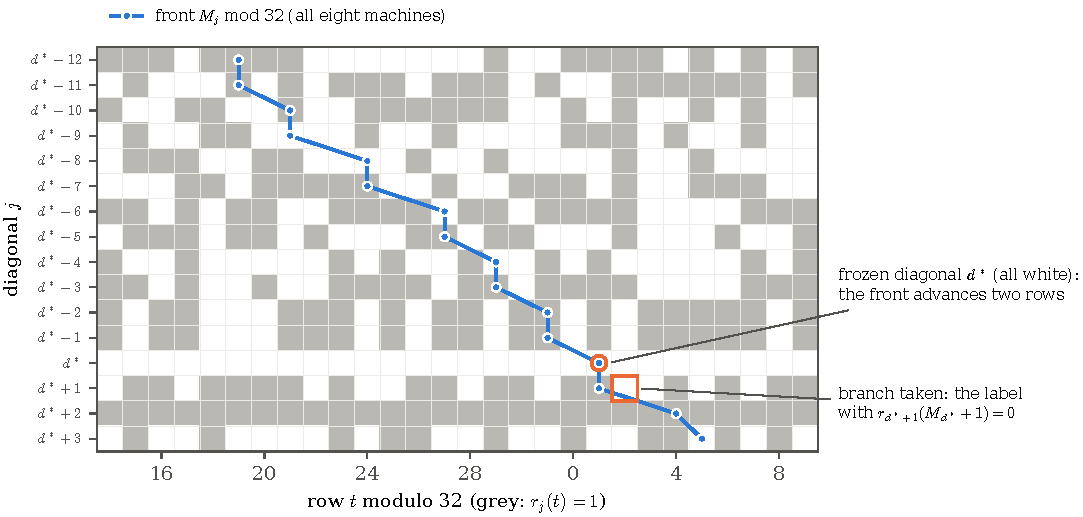
\includegraphics[width=0.9\textwidth]{figures/fig_fork_path.pdf}
\caption{The front's path through the labels at the eighth frozen diagonal $\dstar=1{,}420{,}878{,}968$. Rows are diagonals $j$, columns are rows $t$ modulo $32$, grey cells are $r_j(t)=1$. Each move from diagonal $j-1$ to $j$ lands on the first grey cell of row $j-1$ after the previous front, as the landing rule requires. The frozen diagonal is all white; the front advances there from $31$ to $1$ (Theorem~\ref{thm:advance}), and the branch taken is the candidate that is white in the cell after the new front (square).}
\label{fig:path}
\end{figure}

\begin{theorem}[the seed's branch at $\dstar$; \PROVED\ given the front's path]\label{thm:seedbranch}
Suppose that, as in each of the eight recorded machines of Computation~\ref{comp:vote}, $M_{\dstar-3}\equiv29$ modulo $32$, the front moves at $\dstar-2$, and $M_{\dstar-1}=M_{\dstar-2}$. Then the front advances at $\dstar$, and the seed's branch is \texttt{6cbda353}, the one on which the period doubles at $2{,}107{,}985{,}255$.
\end{theorem}

\begin{proof}
Write $d=\dstar$. The label cells used are $r_{d-3}(30)=0$, $r_{d-3}(31)=1$, $r_{d-2}(31)=1$, $r_{d-1}(0)=0$ and $r_{d-1}(1)=1$ (rows modulo $32$), read from $r_{d-3}=\texttt{b792cb87}$ and $r_{d-2}=r_{d-1}=\texttt{dae372fa}$. By the landing rule the move at $d-2$ goes from $M_{d-3}$ to the next black cell of $r_{d-3}$, which is $M_{d-3}+2$. So $M_{d-2}=M_{d-1}=m$ with $m=M_{d-3}+2\equiv31$.
\begin{enumerate}[leftmargin=*,itemsep=1pt]
\item $D_{d-2}(m)=\neg r_{d-2}(m)=0$: the defect at the landing row of the move at $d-2$ (Lemma~\ref{lem:front}(d)).
\item $D_{d-1}(m+1)=r_{d-1}(m+1)=r_{d-1}(0)=0$, since row $m+1$ lies beyond the front $M_{d-1}=m$.
\item $D_{d-3}(m)=r_{d-3}(m)=1$, since row $m$ lies beyond the front $M_{d-3}=m-2$.
\item By \eqref{eq:frame} on diagonal $d-1$: $0=D_{d-1}(m+1)=D_{d-3}(m)\oplus(D_{d-2}(m)\vee D_{d-1}(m))=1\oplus D_{d-1}(m)$, so $D_{d-1}(m)=1$.
\item By \eqref{eq:frame} on diagonal $d$: $D_d(m+1)=D_{d-2}(m)\oplus(D_{d-1}(m)\vee D_d(m))=0\oplus1=1$.
\end{enumerate}
By Theorem~\ref{thm:advance} the front advances to the first black cell of $r_{d-1}$ at or after row $m+1\equiv0$, which is $m+2\equiv1$, and the branch has $r_{d+1}(m+3)=r_{d+1}(2)=0$. Bit $2$ of \texttt{6cbda353} is $0$ and bit $2$ of \texttt{93425cac} is $1$.
\end{proof}

\begin{remark}[the wall alone does not decide; \EXACT]\label{rem:census}
Take every front history of depth $8$ before $\dstar$ that is consistent with the landing rule, from every starting phase. Propagating \eqref{eq:frame} as a constraint from the known cells (every label cell beyond its front, and the defect at each landing row), as in the proof of Theorem~\ref{thm:seedbranch}, forces an advance for $1{,}038$ of the $4{,}096$ histories, a stall for $1{,}791$, and neither for $1{,}267$. Both verdicts occur, at depth $5$, at every frozen diagonal of the seed from $28$ to $87{,}866$. So at none of these frozen diagonals does the wall alone decide the branch: paths of the front that are all consistent with it force different branches. Nor does the path always decide it: at $28$ and $58{,}286$ the seed's own advance is not forced by this propagation at any depth up to $32$, and there the transient decides. The hypothesis of Theorem~\ref{thm:seedbranch} is a statement about the front's path, which is measured, not proved.
\end{remark}

\begin{remark}[the doubling itself; \EXACT]\label{rem:doubling}
Eight coin-driven machines, started $2\cdot10^6$ diagonals before $2{,}107{,}985{,}254$, all stall there. Their branches split four to four, because the candidates \texttt{b6e14797\allowbreak 491eb868} and \texttt{491eb868\allowbreak b6e14797} (bit $t$ of the $64$-bit word is the cell on row $t$ modulo $64$) are translates by $32$ rows and each machine picks by its front row modulo $64$. Seven of the eight share one front history modulo $32$, a move to row $8$ modulo $32$ five diagonals before the doubling and then stalls, a case Theorem~\ref{thm:advance} does not cover; the eighth is at row $26$. Seen from the front, the seven take the same label, so which translate the seed takes is decided by its front row modulo $64$, and no datum of the period-$32$ wall fixes that. So the absolute phase of the seed's period-$64$ wall is one bit the recursion cannot supply. Frozen diagonals, forks and everything measured relative to the front do not depend on it.
\end{remark}

\section{What the wall alone produces}

The labels define a centre column of their own, $b_B(t)=r_t(t)$: the cell the stripes would put on the centre column if every diagonal were periodic from the start. Lemma~\ref{lem:rec} computes it without the rule, $10^9$ bits in $35$ seconds.

\MEASURED: $b_B$ passes every fair-coin test we applied to $10^9$ bits but one. Its density is $0.500029$, its run counts for lengths $1$ to $12$ are within $1.3$ standard deviations of a coin's, and the $\chi^2$ of its blocks of length $8$, $12$ and $16$ lie $1.5$, $0.3$ and $0.2$ standard deviations below a coin's mean. No context of up to $16$ bits predicts it better than a coin does; that test was calibrated against a coin and against the real column at equal length. It has no period up to $10^7$ on its last $10^8$ bits. At the $26$ lags we tested between $1$ and $128$ its autocorrelation is within $2.1$ standard deviations of zero, except at lag $64$, where it is $6.2$ standard deviations below, a trace of the period-$32$ stripes; this is the one test it fails. On rows $90{,}001$--$1{,}130{,}000$ it agrees with the real centre column $c$ on a fraction $0.49973$ ($z=-0.55$).

\begin{proposition}[decomposition; \PROVED, with a \MEASURED\ reading]
$c(t)=b_B(t)\oplus\Delta_t(t)$ for every $t$. On rows $1{,}000$--$1{,}130{,}000$ the transient bit $\Delta_t(t)$ behaves as a fair coin: density $0.50015$, the $2\times2$ table of $c$ against $b_B$ flat to $10^{-3}$, and every conditional frequency we measured within $2.1$ standard deviations of $\tfrac12$: given the wall's phase ($t$ modulo $16$, $32$ or $64$), the three wall cells around it, the distance to the next black cell of $r_t$, the period, whether the front moves at diagonal $t$, how far row $t$ is from the front, and the mode of the defect there.
\end{proposition}

The identity is immediate, since $D_t(t)=u^t_0=c(t)$. For every $t$ from $20$ to $800{,}000$, $\tau_t>t$: row $t$ lies in the transient of diagonal $t$, so $\Delta_t(t)$ is a live transient bit (the front row, $M_t\approx1.32\,t$, is far past it). That this persists for all $t$ is, up to one row, the conjecture that $\tau_d\ge d$ for every $d\ge20$ (Conjecture~H of \cite{B}; \EXACT\ to $d=4\cdot10^6$, \OPEN\ beyond), which says that the stripes never cross the centre column. The centre column is therefore a sequence the wall computes, XOR a transient bit on which, as far as measured, nothing the stripes know has any influence.

\section{The front: speed and stalls}

\MEASURED: in the coin-driven edge machine the front advances $1.321294$ rows per diagonal on the seed's period-$32$ wall, the mean of twenty runs over $2.8\cdot10^{10}$ diagonals in all (spread between runs $0.000019$, error of the mean $0.000004$), and $1.321438$ on the period-$64$ wall, four runs over $1.2\cdot10^{10}$ (spread $0.000007$). On each block of $10^8$ diagonals the twenty coins agree to within $0.0001$ (standard deviation), while the twenty-run means of different blocks vary with standard deviation $0.00013$, seven times what the coins alone would give, so the speed is a property of the wall. On period-$16$ walls it is about $1.333$. The stall lengths have one geometric tail at both periods, with ratio $0.433$ at period $32$ and $0.434$ at period $64$. Leaving out the one stall at the start of each run, while the transient fills in from the crystal start, the longest stalls seen are $24$ at period $32$ and $26$ at period $64$, against $P-1=31$ and $63$. Extrapolating the tail, a stall of $32$ is expected once per $2.7\cdot10^{12}$ diagonals and one of $64$ once per $10^{24}$. This is the margin of the empirical bound $k_i\le P_i-1$ on the length $k_i$ of the $i$th run of consecutive stalls, $P_i$ the period there, which holds on the seed exactly up to diagonal $800{,}000$ \cite{B}. In \cite{B} we prove that $\tau_d\ge d$ for all $d\ge20$ follows from the finite check $\tau_d\ge d$ for $20\le d\le36$ together with two inequalities on the front holding from diagonal $36$ on: one on the stall runs, $k_i\le\sigma_i-d_i-P_i+1$ with $\sigma_i$ the row and $d_i$ the diagonal at which the run begins, which asks much less than $k_i\le P_i-1$ once the slack $\sigma_i-d_i$ is large (on the seed's data it grows like $0.32\,d_i$, so a stall run would have to last about $0.32\,d_i-P_i$ diagonals to violate it); and one on a second quantity, the cancellation depth of the defects, checked exactly to $800{,}000$ there and not addressed here.

\section{Open problems}

Each of the following is \OPEN.
\begin{enumerate}[leftmargin=*,itemsep=1pt]
\item \emph{The front's path at $\dstar$.} Prove that the seed's front has the path the coin-driven models show, $M_{\dstar-3}\equiv29$ modulo $32$, a move, then a stall. This makes Theorem~\ref{thm:seedbranch} unconditional. More generally, explain why fronts driven by independent coins keep one phase against the wall (Computation~\ref{comp:vote}), although the wall alone does not fix the branch (Remark~\ref{rem:census}).
\item \emph{The fork law.} Prove that the distance between consecutive labels is asymptotically binomial within each regime, or only that frozen diagonals occur at rate $2^{-P(1+o(1))}$.
\item \emph{The transient bit.} Prove anything about $\Delta_t(t)$ jointly with $b_B(t)$. Since $c(t)=b_B(t)\oplus\Delta_t(t)$ and $b_B$ is computable, every statistical question about the centre column is one about this pair.
\end{enumerate}

\section*{Data and code}

All code, data and logs are in the accompanying repository:
\begin{center}\url{https://github.com/nateberzai-svg/rule30-left-edge}\end{center}
\begin{sloppypar}
\begin{itemize}[leftmargin=*,itemsep=1pt]
\item The recursion: \path{scripts/wall_recursion.c} and \path{scripts/wall_recursion128.c}; logs, including the frontier run and the second machine's checkpoints, in \path{results/wall_recursion_logs}.
\item The edge machine: \path{scripts/edge_machine.c}; runs in \path{results/edge_machine_runs}.
\item The fork law: \path{scripts/label_distance.c}; logs in \path{results/fork_law}.
\item Theorem~\ref{thm:seedbranch} and Remarks~\ref{rem:census}--\ref{rem:doubling}: \path{scripts/stall_lookback_trace.py} and \path{scripts/stall_census.py}; labels and machine logs in \path{results/fork_mechanism}.
\item Section~7: \path{scripts/frozen_column.py} and \path{scripts/frozen_column_autocorr.py}; logs in \path{results/frozen_column}.
\item The figures: \path{paper/figures/make_figures.py}.
\item \path{paper/verify_claims.py} recomputes every number stated here from the labels to $800{,}000$ in \path{paper/data} and from the logs, and prints each claim with the value it finds.
\end{itemize}
\end{sloppypar}

\begin{thebibliography}{9}
\bibitem{B} N.~Berzai, The centre column of Rule~30: excluded periods, decimation of the Duhamel class, and the front of the diagonal defects, manuscript, 2026; \texttt{paper/RULE30\_PAPER.pdf} in the repository above.
\bibitem{Dib} Dibujaron (D.~McPolstra), \emph{rule30}, code repository, commit \texttt{94833d2} of 8 September 2026: \path{blueprint/crystals.md}, item~55, \path{explorer/orbit32.mjs}, and the note of that date on the left-diagonal periods in \path{docs/attacks}, claim~C4; \url{https://github.com/Dibujaron/rule30/commit/94833d21c1efc1e826df3c137777b580817c5e16}.
\bibitem{GG} J.~Gravner, D.~Griffeath, Robust periodic solutions and evolution from seeds in one-dimensional edge cellular automata, \emph{Theoret.\ Comput.\ Sci.} 466 (2012) 64--86.
\bibitem{Jen86} E.~Jen, Global properties of cellular automata, \emph{J.\ Stat.\ Phys.} 43 (1986) 219--242.
\bibitem{Pat} Patto1155, \emph{rule30-foundry}, code repository, commit \texttt{04f30f6} (pull request~32) of 8 September 2026, from a run of about 30 August 2026: the log of 8 September 2026 in \path{docs/experiment-logs} and the run file in \path{runs/b1-recovered-2026-09-08}; \url{https://github.com/Patto1155/rule30-foundry/commit/04f30f6085210b476e64d742c77dc7c69a075791}. The log of 9 September 2026 in the same folder is from commit \texttt{1afaa25} of that date.
\bibitem{Rowland} E.~S.~Rowland, Local nested structure in Rule 30, \emph{Complex Systems} 16 (2006) 239--258.
\bibitem{Lania} szymon-lania, Starting state for rule 30 that produces ``the other'' version of diagonal 53209, gist, 21 August 2026, described in its author's comment on E.~Rowland's video \emph{The Hidden Structure of Rule 30}; \url{https://gist.github.com/szymon-lania/2535d62468a7912137b5002d900ebdd6} and \url{https://www.youtube.com/watch?v=HcGjCcLEgN4}.
\bibitem{NKS} S.~Wolfram, \emph{A New Kind of Science}, Wolfram Media, 2002.
\end{thebibliography}

\end{document}
